\documentclass[titlepage, a4paper]{article}
\usepackage[english]{babel}
\usepackage[utf8]{inputenc}
\usepackage{graphicx}
\usepackage{color}
\usepackage{mathtools}
\usepackage{float}
\usepackage[parfill]{parskip}
\usepackage[margin=10pt,font=small,labelfont=bf,labelsep=endash]{caption}
\usepackage{epstopdf}
\usepackage{listings}
\epstopdfsetup{suffix=}
\DeclareGraphicsExtensions{.ps}
\DeclareGraphicsRule{.ps}{pdf}{.pdf}{`ps2pdf -dEPSCrop -dNOSAFER #1 \noexpand\OutputFile}

\lstset{literate=%
    {å}{{\r{a}}}1
    {ä}{{\"a}}1
    {ö}{{\"o}}1
    {Å}{{\r{A}}}1
    {Ä}{{\"A}}1
    {Ö}{{\"O}}1
}

\newcommand{\todo}[1] {\textbf{\textcolor{red}{#1}}}

\usepackage{fancyhdr}
\fancyhead[L]{}
\pagestyle{fancy}
\rhead{Pål Kastman \\ Alexander Yngve}
\chead{TDTS08}
\thispagestyle{empty}

\begin{document}

{\ }\vspace{45mm}

\begin{center}
  \Huge \textbf{TDTS08: whattolearn}
\end{center}

\vspace{250pt}

\begin{center}
  \begin{tabular}{|*{3}{p{40mm}|}}
    \hline
    \textbf{Name} & \textbf{PIN} & \textbf{Email} \\ \hline
           {Pål Kastman} & {851212-7575} & {palka285@student.liu.se} \\ \hline
           {Alexander Yngve} & {930320-6651} & {aleyn573@student.liu.se} \\ \hline
  \end{tabular}
\end{center}
\newpage

\tableofcontents
\thispagestyle{empty}
\newpage

\section{Introduction}
This documents only purpose is to document what I will need to learn in the course tdts08. \\
\todo{YNGVE OM DU VILL BYTA RUBRIKERNA SÅ ÄR DET HELT OKEJ, DOM ÄR BARA DÄR SOM STÖD NU}

\section{Lecture 1: Memory Systems}
\textbf{Memory hierarchy} \\
registers, cache, main memory etc.

\subsection{Cache memory}
how does it work? why do we use it? positive and negative things about it!

\subsubsection{Locality of reference}
Temporal- and spatial locality, differences and how we use these in caches.

\subsubsection{Replacement methods}
yes, there's different kinds of them.

\subsubsection{Cache Design}
One, two, three level caches, how does it work. up- and downsides of them.

\subsubsection{Split Caches}

\subsubsection{Unified Caches}

\subsubsection{Direct mapping cache}

\subsubsection{Associative mapping cache}

\subsubsection{Fully Associative Organization}

\subsubsection{Write Policy}
\textbf{Write through} \\
\textbf{Write through with buffered write} \\
\textbf{Write back} \\

\subsection{Virtual memory}
\subsubsection{Paging}
\subsubsection{Page fault}
\subsubsection{Page replacement}
\subsubsection{Replacement algorithms}

\section{Lecture 3: Instruction pipelining}
how does it work, and why do we need it?

\subsection{Pipeline hazards}
what problems do we have with pipelining

\subsubsection{Structural (resource) hazards}
what are they and how do we solve it?

\subsubsection{Data hazards}

\subsubsection{Control hazards}

\subsection{Branch handling}
\subsubsection{Pre-fetch branch target}
\subsubsection{Loop buffer}
\subsubsection{Delayed branch}

\subsection{Branch prediction}
\subsubsection{Static Branch Prediction}
\subsubsection{Dynamic Branch Prediction}
\subsubsection{Bimodal Prediction}

\section{Lecture 4: RISC Computers}
What are they, how do they work, and why do we need them? \\
Semantic gap \\
Problems with RISC \\

\subsection{Program execution features}
what are programs doing most of the time?

\subsection{RISC characteristics}
Small number of simple instructions \\
Execution of one instruction per clock cycle \\
Complex operations are executed as a sequence of simple instructions \\
only LOAD and STORE instructions reference data in memory \\
Only a few simple addressing modes are used \\
Instructions are of fixed length and uniform format. \\
Large number of registers, this is because the reduced complexity of the processor leaves silicon space on the chip to implement them (opposite of CISC).
\subsubsection{Register Windows}
Large number of registers is usually very useful. \\
However, if contents of all registers must be saved at every procedure call, more registers mean longer delay. \\
A solution to this problem is to divide the register file into a
set of fixed-size windows. \\
-- Each window is assigned to a procedure. \\
-- Windows for adjacent procedures are overlapped to allow parameter passing \\

\subsubsection{Main advantages of RISC}
Best support is given by optimizing most used and most time consuming architecture aspects.\\
-- Frequently executed instructions. \\
-- Simple memory reference. \\
-- Procedure call/return. \\
-- Pipeline design. \\
Consequently, we have: \\
-- High performance for many applications;  \\
-- Less design complexity; \\
-- Reduced power consumption: \\
-- reducing design cost and time-to-market (newer technology) \\

\subsubsection{Criticism of RISC}
Operation might take several instructions to accomplish \\
more memory access might be needed \\
Execution speed may be reduced for certain applications. \\

It usually leads to longer programs, which needs larger memory space to store. \\
It makes it more difficult to program machine codes and assembly programs. \\

\subsection{RISC vs. CISC}
In embedded processors RISC is the better choice

\section{Lecture 5: Superscalar Architecture (SSA)}
Computer designed to improve computation on scalars instructions. \\
A scalar is a variable that can hold only one atomic value at a time, e.g., an integer or a real. \\
A scalar architecture processes one data item at a time -- the computers we discussed up till now. \\
Examples of non-scalar variables: \\
-- Arrays -- Vector Processor \\
-- Matrices -- Graphics Processing Unit (GPU) \\
-- Records \\

In a superscalar architecture (SSA), several scalar instructions can be initiated simulaneously and executed independently.

\subsection{Instruction-level parallelism}
Most operations are on scalar quantities, speed up these operations will lead to large performance improvement.

\subsection{Superpipelining}
Divide pipelining stages into different several sub-stages, and hence increase the number of instructions which are handled by the pipeline at the same time. \\
\todo{A picture would be nice here} \\

-- For example by diving each stage into two sub stages, we will be able (in the ideal situation) to perform each stage at twice the stage. \\
-- No duplication of hardware is needed. \\
-- Not all stages can be divided into (equal length) sub stages. \\
-- Hazards more difficult to resolve. \\
-- More complex hardware. \\
-- Interrupt handling and testing will be more complicated. \\

\subsection{Difference between Superpipelined and Superscalar Designs}
The difference is that Superpipeline can perform several instructions in one clock cycle, whereas Superscalar performs several instructions in parallel

\begin{figure}[H]
  \centering
  \scalebox{0.342}{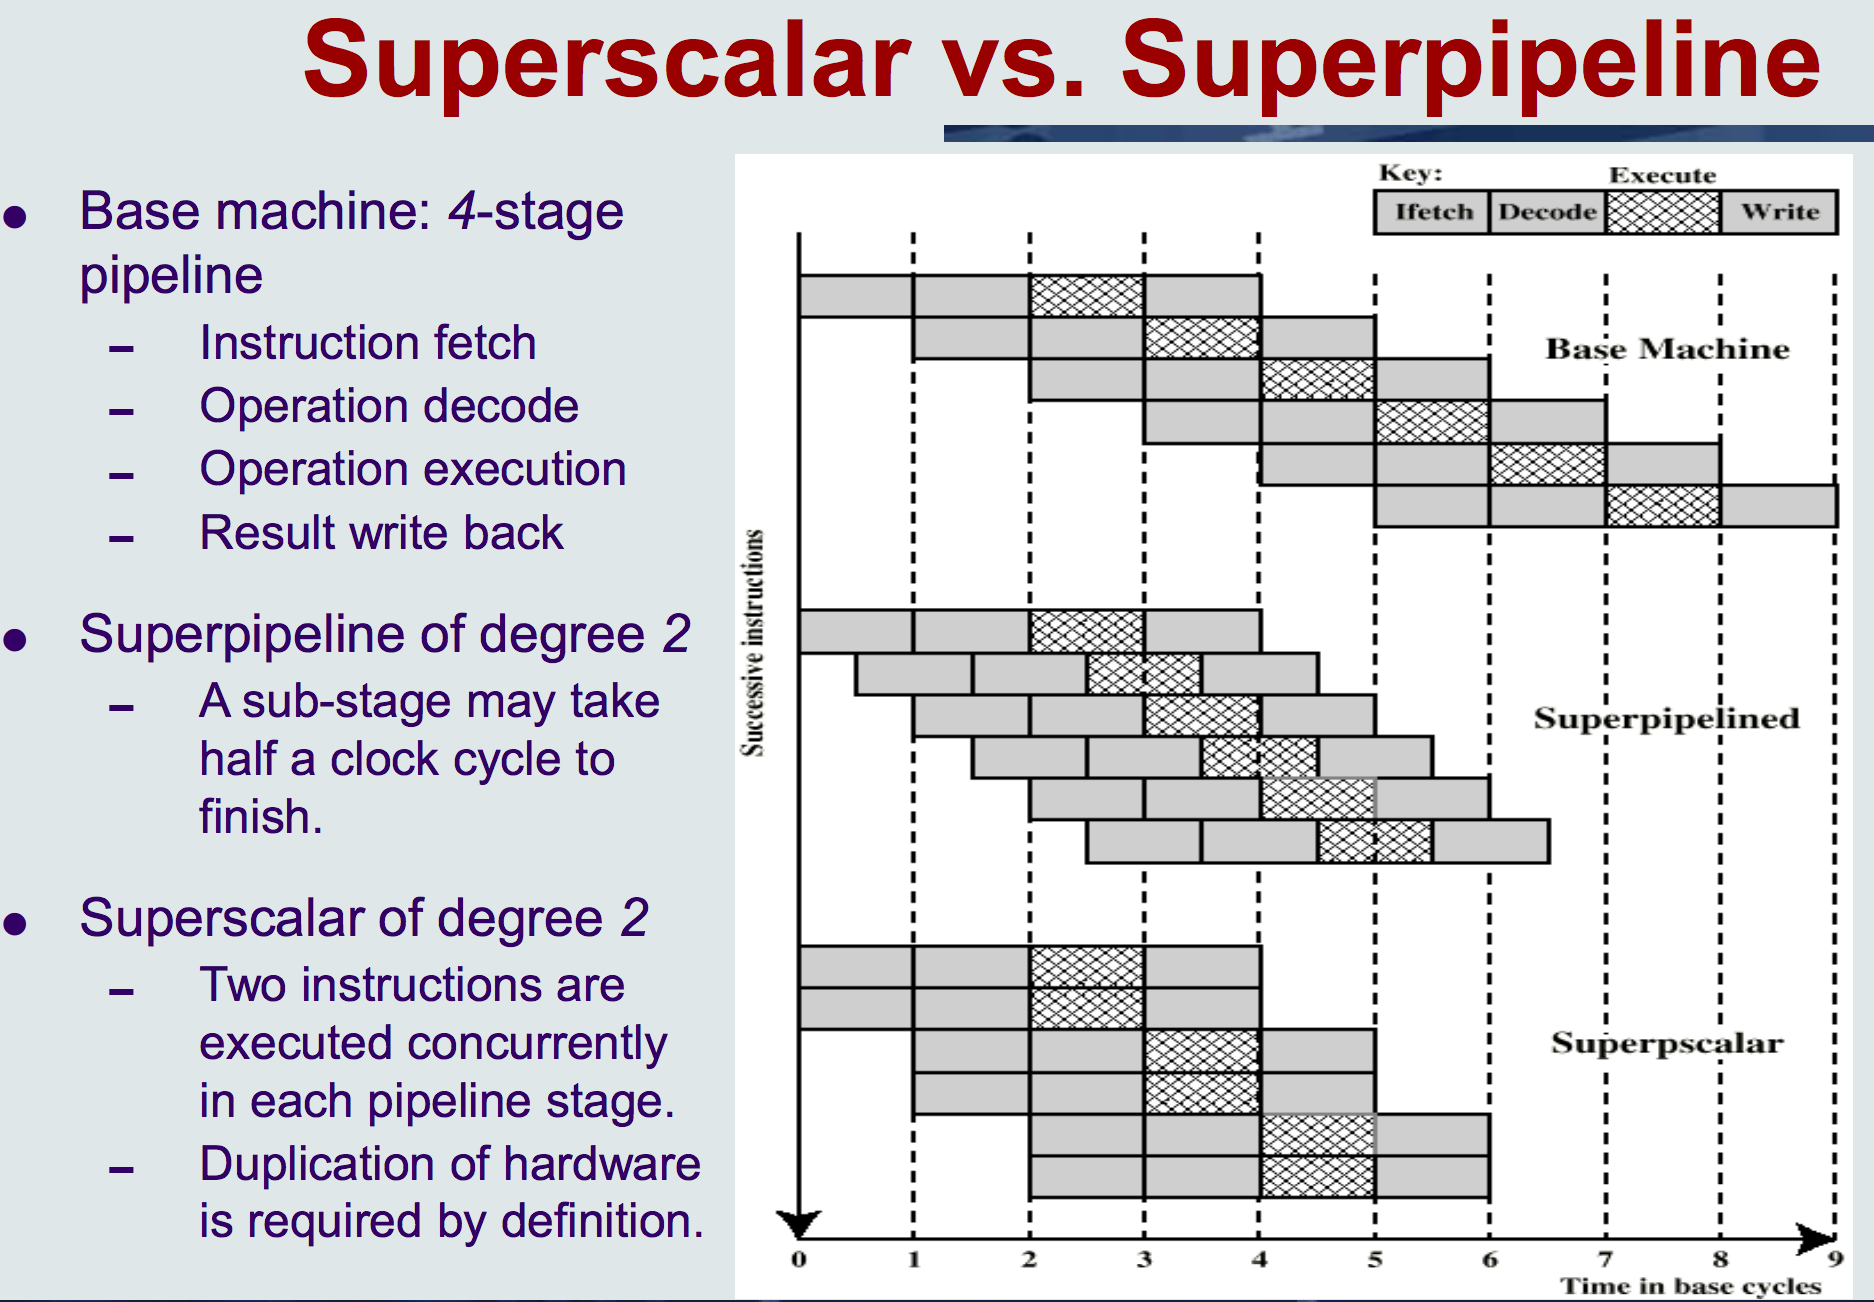
\includegraphics{img/superscalar-vs-superpipeline.png}}
  \caption{Difference between a Superscalar and a Superpipeline architecture}
  \label{fig:superscalar-vs-superpipeline}
\end{figure}


\subsection{Superscalar Superpipeline Design}

\begin{figure}[H]
  \centering
  \scalebox{0.342}{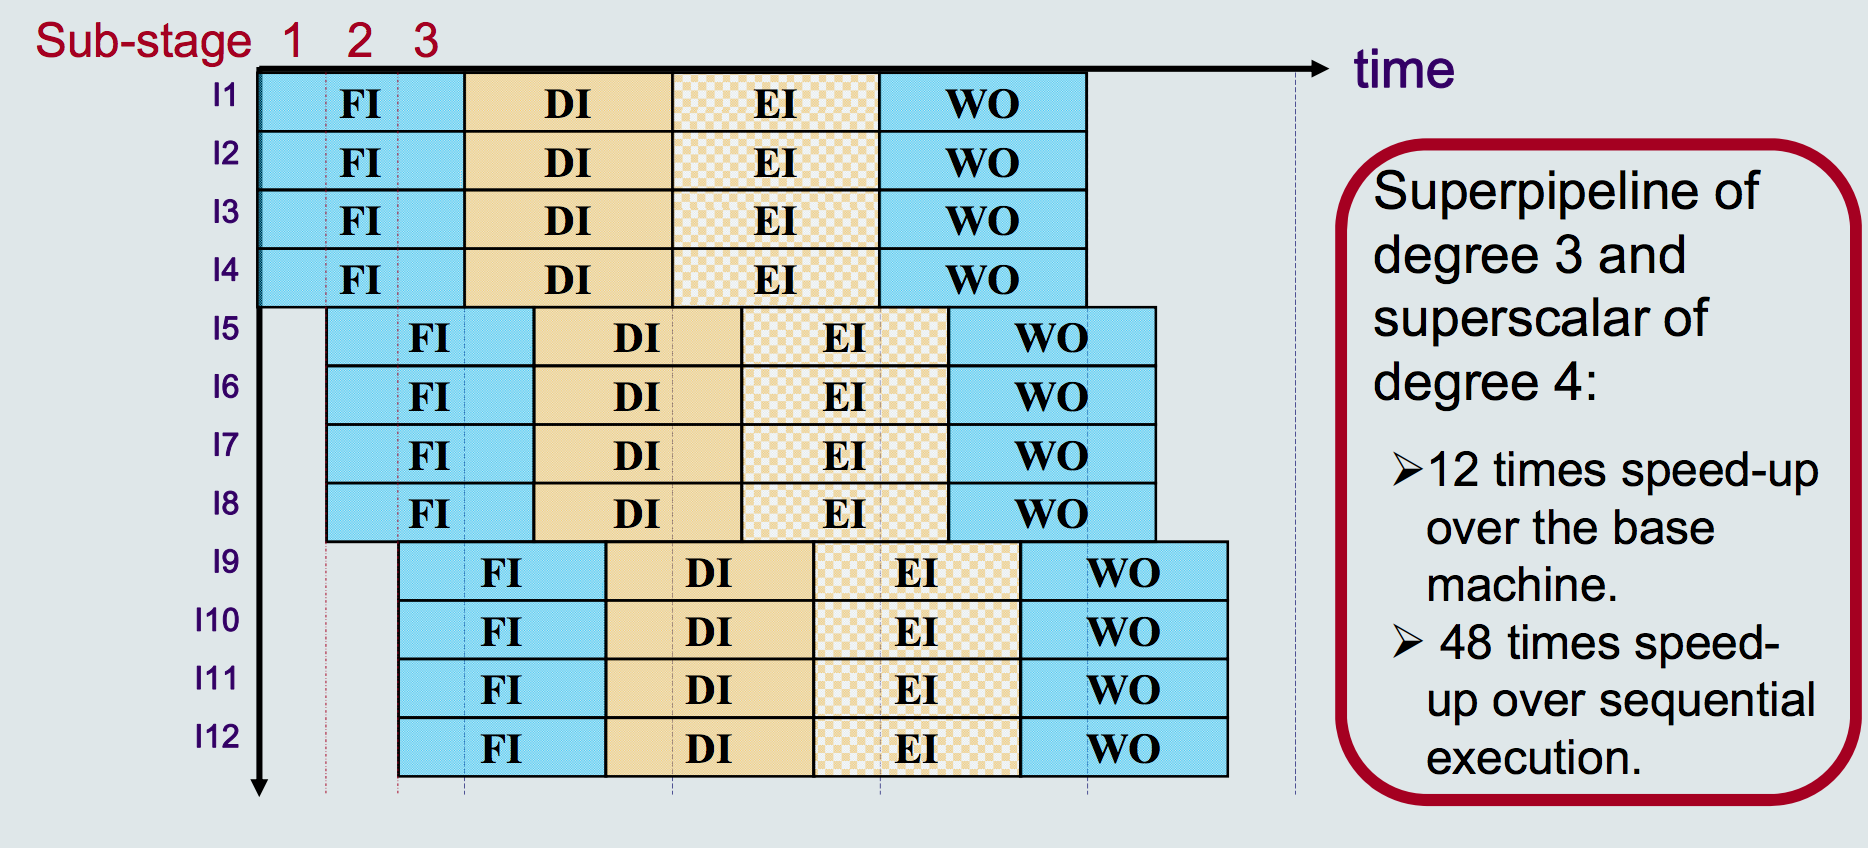
\includegraphics{img/superscalar-superpipeline.png}}
  \caption{Superscalar Superpipeline architecture}
  \label{fig:superscalar-superpipeline}
\end{figure}

The new trend is to combined the two ideas. In Figure \ref{fig:superscalar-superpipeline} it says that this would give us a 48 times speedup, this is not the case though because of data dependencies.

\subsection{Dependency issues}
The main problems are:
-- Resource conflicts. \\
-- Control (procedural) dependency. \\
-- Data dependencies. \\

These are very similar to the cases in normal pipelining (data hazards). But the consequences are more severe here because the parallelism are greater and thus larger amount of performance will be lost. \\

\subsubsection{Resource Conflicts}
Several instructions compete for the same hardware resource at the same time.
-- For instance, two aritmethic instructions need the same floating-point unit for execution. \\
-- similar to structural hazards in pipeline. \\

They can be solved \underline{partly} by introducing several hardware units for the same functions. \\
-- e.g. have two floating point units. \\
-- the hardware units can also be pipelined to support several operations at the same time. \\
-- however, memory units \textbf{can't be duplicated}.

\subsubsection{Procedural Dependency}

\subsubsection{Data Conflicts}

\subsubsection{Window of execution}

\subsubsection{Data Dependency}

\subsubsection{True Data Dependency}

\subsubsection{Output Dependency}

\subsubsection{Anti Dependency}

\subsubsection{Effect of Dependencies}

\subsection{Parallel instruction execution}

\subsubsection{Instruction vs Machine Parallelism}

\subsubsection{Division and Decoupling}

\subsubsection{SSA instruction Execution Policies}

\subsubsection{In-Order with In-Order Completion}
This seems important to understand

\subsubsection{In-Order issue with Out-of-Order Completion}
This seems important to understand

\section{Lecture 6: VLIW Processors}
The difference from Superscalar is that in that architecture the hardware solves everything for us, if improvements are made on the design we don't need to change the programs. \\
The down side though is that the architecture is very complex. \\
-- A lot of hardware is needed for run-time detection of parallelism. \\
-- It consumes a lot of power. \\
-- There is, therefore a limit in how far we can go with this technique. \\

The instruction window for execution is limited in size. \\
-- This limits the capacity to detect large number of parallel instructions.

\subsection{Very Long Instruction Word Processors}
Several operations that can be executed in parallel are placed in a single instruction word. \\
--VLIW rely on compile-time detecton of parallelism. \\
-- The compiler analyzes the program and detects operations to be executed in parallel. \\

After one instruction has been fetched, all the corresponding operations are issued in paralell.
The instruction window limitation disappears: the compiler can potentially analyze the whole program to detect parallel operations.

\subsubsection{Explicit Parallelism}
Instruction parallelism scheduled at compile time.\\
-- Included within the machine instructions explicitly.\\

An EPIC (Explicitly Parallel Instruction Computing) processor \\
--uses this information to perform parallel execution. \\

The hardware is very much simplified \\
-- The controller is similar to a simple scalar computer. \\
-- The number of FUs can be increased without needing additional sophisticated hardware to detect parallelism, as in SSA. \\

Compiler has much more time to determine parallel operations. \\
-- This analysis is only done once off-line, while run-time detection is carried out by SSA hardware for each execution of the code. \\
--Good compilers can detect parallelism based on global analysis of the whole program. \\

\subsubsection{Main issues}
-- Need a large number of registers. \\
-- Large data transport capacity is needed between Fus and the register files and between register files and memory. \\
-- High bandwidth between instruction cache and fetch unit is also needed due to long iunstructions.

\subsubsection{Software issues}

\subsection{Loop unrolling}

\subsection{IA-64 architecture}
\subsubsection{Predicated execution}
\subsubsection{Instruction format}
\subsubsection{Branch Predication}
\textbf{NOT THE SAME AS BRANCH PREDICTION}
\subsubsection{Placement of Loading}
\subsubsection{Speculative Loading}

\section{Parallel Processing}
\subsubsection{Why Parallel Processing?}
\subsubsection{Parallel Computer}
\subsubsection{Parallel Program}

\subsection{Architecture classification}
\subsubsection{Flynn’s Classification of Architectures}
-- Single instruction, single data stream - \textbf{SISD} \\
-- Single instruction, multiple data stream - \textbf{SIMD} \\
-- Multiple instruction, single data stream - \textbf{MISD} \\
-- Multiple instruction, multiple data stream- \textbf{MIMD} \\

\todo{GÅ IGENOM DESSA}\\

\subsection{Performance evaluation}

\subsection{Interconnection network}
\subsubsection{Single Bus}
\subsubsection{Completely Connected Network}
\subsubsection{Crossbar Network}
\subsubsection{Mesh Network}
\subsubsection{Hypercube Network}

\section{Lecture 8: SIMD Architectures}

\subsection{Vector Processors}
-- array processors \\
-- vector processors \\
-- data parallelism \\
Typical SISD processors who behave like SIMD processors

\subsubsection{Instruction-level parallelism}
\subsubsection{Thread-level parallelism}
\subsubsection{Data parallelism}
\subsubsection{Vector Processors}
\subsection{Array Processors}
Typical SIMD processors

\subsection{Dedicated Memory Organization}
\subsection{Global Memory Organization}
\subsection{Cray supercomputers}
\subsubsection{Cray X1}
\subsection{Multimedia extensions}
\subsubsection{sub-word execution}
\subsubsection{Packed Data Types}
\subsubsection{SIMD Arithmetic Examples}

\section{Lecture 9: MIMD Architectures}
A set of general purpose processors connected together \\
In contrast to a SIMD computer, a MIMD computer can execute different programs on different processors. \\

-- Works asynchronously, and don't have to synchronize with each other. \\
-- At any time, different processors may be executing different instructions on different pieces of data. \\
-- They can be built from commodity (off-the-shelf) microprocessors with relatively little effort. \\
-- They are also highly scalable, provided that an appropiate memory organization is used. \\
-- Most current parallel computer are built based on the MIMD architecture. \\

\subsubsection{SIMD vs. MIMD}
\subsubsection{MIMD Processor Classification}
\subsubsection{MIMD with Shared Memory}
\subsubsection{MIMD with Distributed Memory}
\subsubsection{Shared-Address-Space Platforms}
\subsubsection{Multi-Computer Systems}
\subsubsection{MIM Design Issues}
\subsection{Symmetric multiprocessors (SMP)}
\subsubsection{SMP Advantages}
\subsubsection{SMP based on Shared Bus}
\subsubsection{Multi-Port Memory SMP}
\subsubsection{Operation System Issues}
\subsubsection{IBM S/390}
\subsection{NUMA Architecture}
\subsubsection{Memory Access Approaches}
\subsection{Clusters}
\subsubsection{Losely Coupled MIMD - Clusters}
\subsubsection{Clusters benefits}
\subsubsection{Clusters Configurations}
\subsubsection{IBM Blue Gene Supercomputer}
\subsubsection{Parallelizing Computation}
\subsubsection{Google Applications}

\section{Lecture 10: Cache Coherence}
To many section without text seems to bug \LaTeX
\subsection{Introduction}
\subsubsection{Write Through}
\subsubsection{Write Back}
\subsubsection{Software Solutions}
\subsubsection{Hardware Solutions}
\subsection{Directory protocols}
\subsubsection{Cache Coherence Operations}
\subsection{Snoopy protocols}
\subsubsection{Write Invalidate SP}
\subsubsection{Snoopy Cache Organization}
\subsubsection{MESI State Transition Diagram}
\subsubsection{Write Update SP}
\subsubsection{Invalidate vs. Update Protocols}
\subsubsection{Directory vs. Snoopy Schemes}
\subsection{L1-L2 consistence}
\subsubsection{Alpha-Server 4100}

\section{Lecture 11: Multi-Core and GPU}
To many section without text seems to bug \LaTeX
\subsection{Multi-Core Computers}
\subsubsection{Intel Core i7}
\subsubsection{Superscalar vs. Multi-Core}
\subsubsection{Single Core vs. Multi-Core}
\subsubsection{Intel Polaris}
\subsection{Multithreading}
\subsubsection{Thread-Level Parallelism (TLP)}
\subsubsection{Scalar Processor Approaches}
\subsubsection{Superscalar Approaches}
\subsubsection{SMT and Chip Multiprocessing}
\subsubsection{Multithreading Paradigms}
\subsection{Graphic Processing Unit (GPU)}
\subsubsection{CPU vs. GPU}
\subsection{General Purpose GPUs}
\subsubsection{Divergent Execution}
\subsubsection{Reduce Branch Divergence}
\subsubsection{GPUPU}
\subsubsection{NVIDIA Tesla}
\subsubsection{CUDA Programming Language}

\end{document}

